% !TEX buildOnSave = true

\documentclass{scrartcl}
\usepackage{multicol}
\usepackage{enumerate}
% \usepackage{pgfplots}
\usepackage{tikz}
\usepackage{tkz-euclide}
\usetkzobj{all}
\usepackage{amsthm,amsmath}

\theoremstyle{definition}
\newtheorem{problem}{Problem}
\newtheorem*{problem*}{Problem}
\renewcommand{\proofname}{Solution:}

\title{Geometric Applications}
\subtitle{Based on Chapter 7 of Schaum's Outline Series ``Theory and Problems of Differential Equations" by Frank Ayres Jr., and Chapter 11 of ``A Treatise on Differential Equations'' by George Boole.}
\author{F.~J.~Blanco-Silva}

\begin{document}
\maketitle

\section*{Basic considerations about explicit plane curves}
Consider a plane curve given explicitly as $y=f(x)$.  Any point on that curve has coordinates $\big(x,f(x)\big)$.  A few basic questions about tangent lines to this graph:
\begin{center}
\begin{tabular}{ccc}
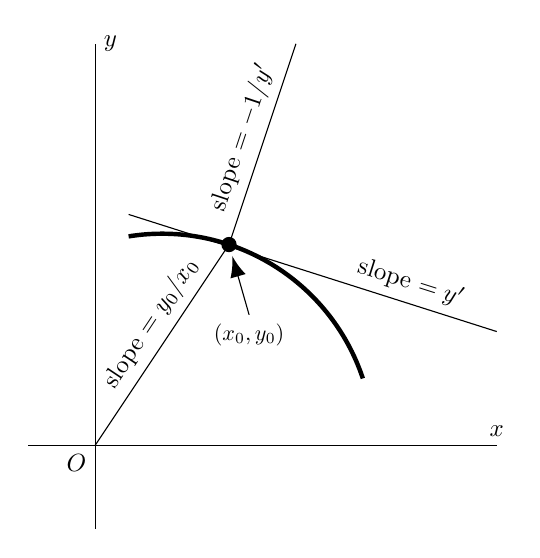
\begin{tikzpicture}[scale=0.85]
\draw (-1,0) -- (6,0) node[scale=0.9,above]{$x$};
\draw (0,-1.25) -- (0,6) node[scale=0.9,right]{$y$};
\draw (0,0) node[scale=0.9,below left]{$O$};
\filldraw (2,3) circle (3pt);
\draw (0,0) -- (2,3) node[scale=0.9, pos=0.55, sloped, above]{slope $= y_0/x_0$};
\draw (2,3) -- (3,6) node[scale=0.9,midway, sloped, above]{slope $=-1/y'$};
\draw (0.5,3.45) -- (6,1.7) node[scale=0.9,near end, sloped, above]{slope $= y'$};
\tkzDefPoint(0.5,3.122){A}\tkzDefPoint(4,1){C}
\tkzDefPoint(1,0){O}
\tkzDrawArc[ultra thick](O,C)(A)
\node (P) at (2,3) {};
\draw[-latex] (2.3,1.95) node[scale=0.8,below]{$(x_0,y_0)$} -- (P);
% center = (1,0)
% radius = sqrt(10)
% (1,0) + sqrt(10) * (\cos\theta, \sin\theta) = (1+\sqrt{10}\cos\theta, \sqrt{10}\sin\theta)
% 1+\sqrt{10}\cos\theta=0.5; \cos\theta=-0.5/\sqrt{10};
% \sin\theta = \sqrt{1-\cos^2\theta} = \sqrt{1-0.5^2/10} = 0.987
% 1+\sqrt{10}\cos\theta=2; \cos\theta=1/\sqrt{10}
% \sin\theta=\sqrt{1-\cos^2\theta}=\sqrt{1-1/10}=\sqrt{9/10}=3/\sqrt{10} yup
% 1+\sqrt{10}\cos\theta=4; \cos\theta=3/\sqrt{10}
% \sin\theta=\sqrt{1-\cos^2\theta}=\sqrt{1-9/10}=1/\sqrt{10}
\end{tikzpicture} & \hspace{0.15cm} &
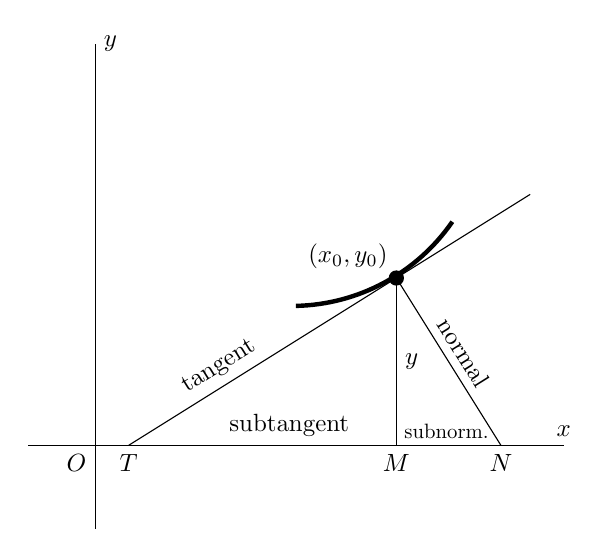
\begin{tikzpicture}[scale=0.85]
\draw (-1,0) -- (7,0) node[scale=0.9,above]{$x$};
\draw (0,-1.25) -- (0,6) node[scale=0.9,right]{$y$};
\draw (0,0) node[scale=0.9,below left]{$O$};
\draw (0.5,0) node[scale=0.9,below]{$T$} -- (6.5,3.75) node[scale=0.9,near start, above, sloped]{tangent};
\draw (6.0625,0) node[scale=0.9,below]{$N$} -- (4.5,2.5) node[scale=0.9,midway,sloped,above]{normal};
\draw (4.5,0) node[scale=0.9,below]{$M$} -- (4.5, 2.5) node[scale=0.9,midway,right]{$y$};
\filldraw (4.5, 2.5) circle (3pt) node[scale=0.9,above left]{$(x_0,y_0)$};
\draw (0.5,0) -- (4.5,0) node[scale=0.9,above,pos=0.6]{subtangent};
\draw (4.5,0) -- (6,0) node[midway, above, scale=0.75]{subnorm.};
% (6.0625, 0) - (4.5,2.5) = (1.5625, -2.5)
% (4.5, 2.5) - (1.5625. -2.5) = (2.9375,5)
% \sqrt(1.5625^2+2.5^2)
\tkzDefPoint(2.9375,5){Q}
% (2.9375,5) + 2.9481191038(\cos\theta, \sin\theta)
% 2.9375+2.9481191038\cos\theta = 3; \cos\theta = 0.0625/2.9481191038 = 0.0211999576
% 5-2.9481191038\sin\theta = 5 - 2.9481191038\sqrt(1-\cos^2\theta) = 2.0832983001
\tkzDefPoint(3,2.0832983001){B}
% 2.9375+2.9481191038\cos\theta = 5; \cos\theta = 2.0518808962/2.9481191038= 0.695996608
% 5-2.9481191038\sin\theta = 5 - 2.9481191038\sqrt(1-\cos^2\theta) = 2.8831176136
\tkzDefPoint(6,2.8831176136){D}
\tkzDrawArc[ultra thick](Q,B)(D)
\end{tikzpicture}
\end{tabular}
\end{center}

\begin{itemize}
\item The slope of the tangent line to the curve at $(x_0,y_0)$ is $f'(x_0)$.
\item The slope of the normal line to the cure at $(x_0,y_0)$ is $-1/f'(x_0)$.
\item The equation of the tangent line at $(x_0,y_0)$ is $y-y_0=y'(x-x_0)$.
\item The equation of the normal line at $(x_0,y_0)$ is $y-y_0 = (x_0-x)/f'(x_0)$.
\item The $x$--intercept of the tangent is $x_0-f(x_0)/f'(x_0)$.
\item The $y$--intercept of the tangent is $f(x_0)-x_0 f'(x_0)$.
\item The $x$--intercept of the normal is $x_0+y_0y'$.
\item The $y$--intercept of the normal is $f(x_0)+x_0/f'(x_0)$.
\item The length of the tangent between $(x_0,y_0)$ and the $x$--axis is $\lvert y_0 \rvert\sqrt{1+1/f'(x_0)^2}$.
\item The length of the tangent between $(x_0,y_0)$ and the $y$--axis is $\lvert x_0 \rvert\sqrt{1+f'(x_0)^2}$.
\item The length of the normal between $(x_0,y_0)$ and the $x$--axis is $\lvert y_0 \rvert\sqrt{1+f'(x_0)^2}$.
\item The length of the normal between $(x_0,y_0)$ and the $y$--axis is $\lvert x_0 \rvert \sqrt{1+1/f'(x_0)^2}$.
\item The length of the subtangent is $\lvert f(x_0)/f'(x_0) \rvert$.
\item The length of the subnormal is $\lvert f(x_0) f'(x_0) \rvert$.
\end{itemize}


\section*{Solved Problems}
\begin{problem*}
At each point $(x,y)$ of a curve, the intercept of the tangent on the $y$--axis is equal to $2xy^2$.  Find the curve.
\end{problem*}

% \begin{center}
% \begin{tikzpicture}[scale=3]
% \draw[step=0.1, gray, ultra thin] (-0.6, -0.45) grid[] (1.25, 0.85);
% \draw[step=0.5, gray, thin] (-0.6, -0.45) grid[] (1.25, 0.85);
% \draw[thick] (-0.6,0) -- (1.25, 0);
% \draw[thick] (0,-0.45) -- (0,0.85);
% \draw[domain=-0.6:1.25,smooth,variable=\x,red, thick]  plot ({\x},{\x/(1+\x*\x)});
% \draw[blue, thick] (-0.6, 0.24) -- (1.25,0.57);
% \filldraw (0.75,0.48) circle (0.25pt);
% \end{tikzpicture}
% \end{center}

\begin{proof}
We are looking for a curve $y=f(x)$ that satisfies $y-xy'=2xy^2$.  This is a Bernoulli equation with solution $x-x^2y=Cy$.
\end{proof}

\begin{problem*}
At each point $(x,y)$ of a curve, the subtangent is three times the square of the \emph{abscissa}.  Find the curve if it also passes through the point $(1,e)$.
\end{problem*}

\begin{proof}
This curve satisfies the differential equation $y/y'=3x^2$.  This is a separable differential equation of first order.  The solutions are of the form $3\ln \lvert y \rvert = C- 1/x$.

We are further requiring the solution to an initial value problem with $f(1)=e$.  We have then $C=4$.  The solution is then $y = e^{4/3} e^{-1/3x}$.
\end{proof}


\begin{problem*}
Find the family of curves for which the length of the part of the tangent between the point of contact $(x,y)$ and the $y$--axis is equal to the $y$--intercept of the tangent.
\end{problem*}
\begin{proof}
We need to solve the differential equation
\begin{align*}
x\sqrt{1+(y')^2} &= y-xy'. \\
\intertext{This could also be written as}
x^2 \big( 1 + (y')^2 \big) &= y^2 + x^2(y')^2 - 2xyy', \\
\intertext{which reduces to}
x^2 &= y^2 -2xyy'
\end{align*}
This is a homogeneous differential equation of order one.  Its general solution is
\begin{equation*}
x^2+y^2=Cx.
\end{equation*}
This is a family of circles that go through the origin, each of them with center on the $x$--axis.
\end{proof}

\begin{problem*}
Find the orthogonal trajectories of the hyperbolas $xy=k$.
\end{problem*}
\begin{proof}
The differential equation of the given family is $xy'+y=0$, obtained by implicit differentiation of the expression $xy=k$ with respect to $x$.  The differential equation of the orthogonal trajectories, obtaining by replacing $y'$ with $-1/y'$ is then (written as an exact differential equation) $y\, dy - x\, dx = 0$.

Integrating this expression, we obtain the family of hyperbolas $y^2-x^2=C$.
\end{proof}

\section*{Supplementary Problems}
\begin{problem}
Find the equation of the curve for which
\begin{enumerate}[(i)]
	\item Find all curves with constant subnormals.
	\item The normal at any point $(x,y)$ passes through the origin.
	\item The slope of the tangent at any point $(x,y)$ is half the slope of the line from the origin to the point.
	\item The perpendicular from the origin to the tangent line at any point $(x,y)$ is constant.
	\item Find all curves for which the subtangent at any point $(x,y)$ is equal to the square of the abscissa.
	\item The normal at any point $(x,y)$ and the line joining the origin to that point form an isosceles triangle having the $x$--axis as base.
	\item The part of the normal drawn at point $(x,y)$ between this point and the $x$--axis is bisected by the $y$--axis.
	\item The length of the perpendicular from the origin to a tangent line of the curve is equal to the abscissa of the point of contact $(x,y)$.
\end{enumerate}
\end{problem}

\begin{problem}
Find the orthogonal trajectories of each of the following families of curves:
\begin{multicols}{2}
\begin{enumerate}[(i)]
	\item $x+2y=k$.
	\item $y=kx^n$, $n$ a positive integer.
	\item $y=k/x^n$, $n$ a positive integer.
	\item $x^2+2y^2=k$
	\item Confocal ellipses $\tfrac{x^2}{a^2}+\tfrac{y^2}{a^2-h^2}=1$
	\item $y=Ce^{-2x}$
	\item $y^2 = x^3/(k-x)$
	\item $y=x-1+ke^{-x}$
	\item $y^2 = 2x^2(1-kx)$
\end{enumerate}
\end{multicols}
\end{problem}
\end{document}
